\documentclass[10pt,a4paper]{article}
\usepackage[left=2cm,right=2cm,top=2cm,bottom=2cm]{geometry}
\usepackage[T1]{fontenc}
\usepackage{lmodern}
\usepackage[spanish,es-tabla,es-noquoting]{babel}
\usepackage[dvipsnames]{xcolor}
\usepackage[fleqn]{mathtools}
\usepackage{booktabs}
\usepackage{amsmath}
\usepackage{latexsym}
\usepackage{graphicx}
\usepackage{nccmath}
\usepackage{multicol}
\usepackage{listings}
\usepackage{tasks}
\usepackage{color}
\usepackage{float}
\usepackage{tikz}
\usepackage{csquotes}
\usepackage[backend=biber,style=numeric,sorting=none]{biblatex}
\addbibresource{referencias.bib}

\definecolor{colorIPN}{rgb}{0.5, 0.0,0.13}
\definecolor{colorESCOM}{rgb}{0.0, 0.5,1.0}
\graphicspath{ {imagenes/} }

\begin{document}
%#########################################################
\begin{titlepage}
	\centering
	{ \huge \bfseries \color{colorIPN}{Instituto Politécnico Nacional} \par}
	{ \Large \bfseries  \color{colorESCOM}{Escuela Superior de Cómputo} \par }
	\vspace{1cm}
	{\huge\Large \color{colorIPN}{Web Client and Backend Development Frameworks}.\par}
	\vspace{1.5cm}
	{\huge\Large  \color{colorESCOM}{Instalación del Java Development Kit (JDK)}\par}
		\vspace{2cm}
	{\Large\itshape \color{colorIPN}{Profesor: Dr. José Asunción Enríquez Zárate}\par} \hfill \break
	\vspace{2cm}
	{\Large\itshape \color{colorIPN}{Alumno: Angel Frausto Robles}\par} \hfill \break
	{\Large\itshape \color{colorIPN}{id634296@gmail.com}\par} \hfill \break
	{\Large\itshape \color{colorIPN}{7CM2} \par}
	\vfill
	{\large \color{colorIPN}{\today}\par}
	\vfill
\end{titlepage}

\renewcommand\lstlistingname{Código}

\lstset{
	language=bash,
	basicstyle=\small\ttfamily,
	numbers=left,
	numberstyle=\tiny,
	frame=tb,
	tabsize=4,
	columns=fixed,
	showstringspaces=false,
	showtabs=false,
	keepspaces,
	commentstyle=\color{Violet},
	keywordstyle=\color{colorIPN} \bfseries,
	stringstyle=\color{colorESCOM},
	extendedchars=true,
	inputencoding=utf8,
	literate=
		{á}{{\'a}}1 {é}{{\'e}}1 {í}{{\'i}}1 {ó}{{\'o}}1 {ú}{{\'u}}1
		{Á}{{\'A}}1 {É}{{\'E}}1 {Í}{{\'I}}1 {Ó}{{\'O}}1 {Ú}{{\'U}}1
		{ñ}{{\~n}}1 {Ñ}{{\~N}}1 {ü}{{\"u}}1 {¿}{{?`}}1 {¡}{{!`}}1
}

\settasks{
	counter-format=(tsk[r]),
	label-width=4ex
}
\tableofcontents
\pagebreak
\listoffigures
\pagenumbering {arabic}

\pagebreak

%################################################
\section{\color{colorIPN}{Introducción}}

El Java Development Kit (JDK) es el paquete de herramientas que permite escribir, compilar y ejecutar programas en el lenguaje Java. Incluye, entre otras piezas, el compilador (\texttt{javac}), la máquina virtual de Java (\texttt{java}) y las bibliotecas estándar del lenguaje. Sin un JDK instalado, un proyecto Java no puede ni siquiera compilarse, y esa es la razón por la que su instalación es el primer paso obligatorio antes de trabajar con cualquier framework construido sobre Java, entre ellos Spring, que sostiene la parte de backend de este curso.

Java como especificación es propiedad de Oracle Corporation \cite{oracle2024jdk}, que además distribuye su propia implementación del JDK. Sin embargo, existen otras distribuciones que implementan la misma especificación y pasan el mismo conjunto de pruebas de compatibilidad (TCK), entre ellas Eclipse Temurin, mantenida por la fundación Eclipse Adoptium \cite{adoptium2024}. Es la distribución que se documenta en este reporte.

El objetivo de este reporte es doble: identificar cuál es la variable de entorno que Java necesita para operar correctamente (\texttt{JAVA\_HOME}) y documentar el proceso completo de descarga, instalación y configuración de esa variable en el sistema operativo, dejando evidencia de cada paso y de la verificación final.

%################################################
\section{\color{colorIPN}{Desarrollo}}

\subsection{ \color{colorESCOM}{Descarga del JDK}}

\begin{figure}[H]
	\centering
	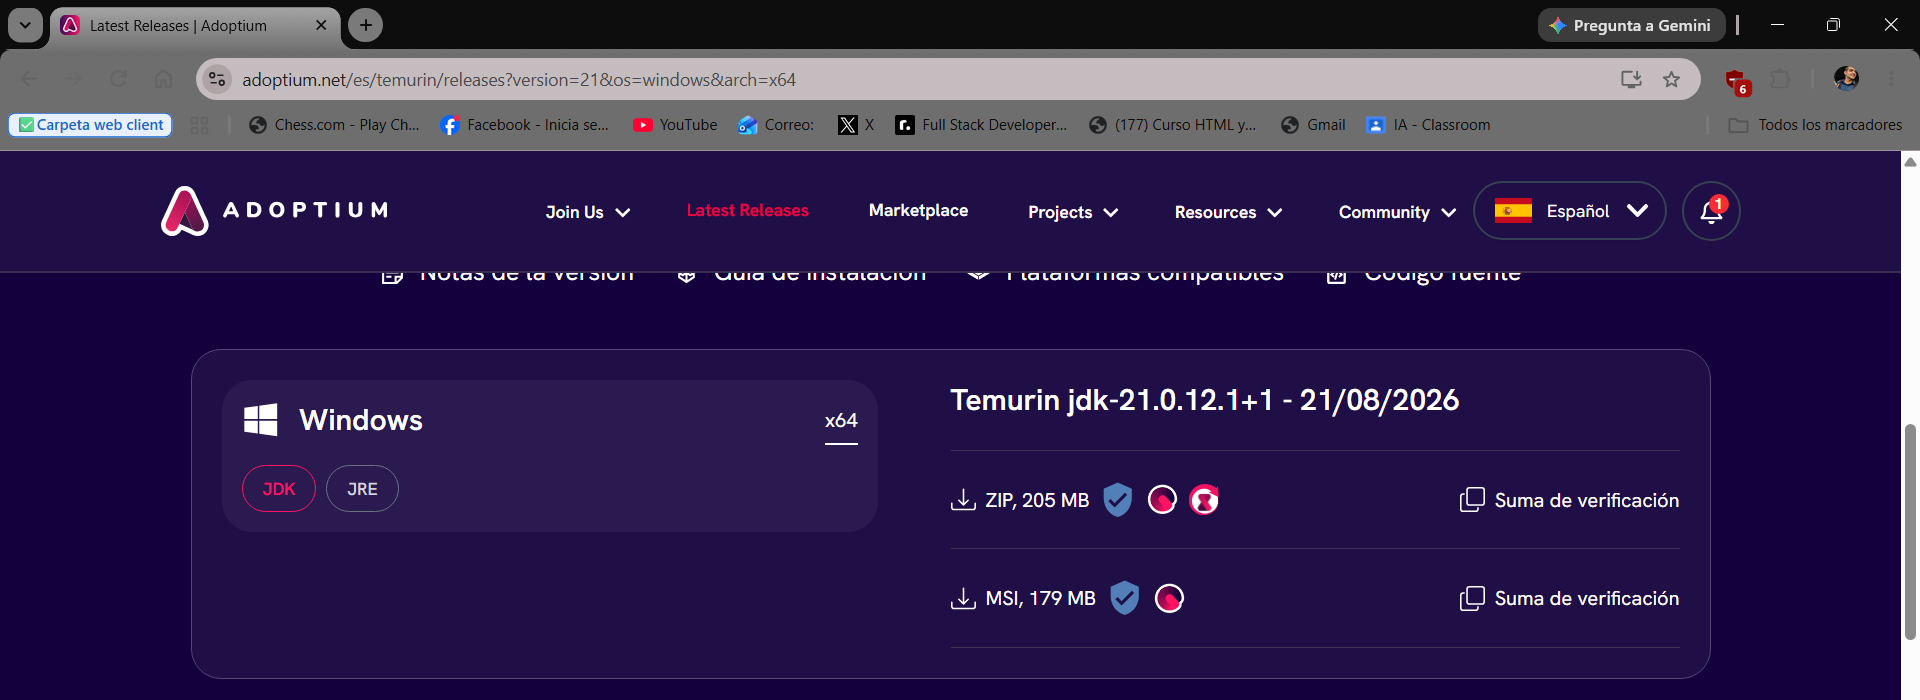
\includegraphics[width=0.85\textwidth]{captura1-descarga.png}
	\caption{Página de descarga del JDK}
	\label{img:descarga}
\end{figure}

El JDK se descargó del sitio oficial de la distribución elegida \cite{adoptium2024}, seleccionando la versión de soporte extendido (LTS) más reciente disponible para el sistema operativo de la máquina de trabajo (Windows, arquitectura x64). Optar por una versión LTS, en vez de una versión intermedia de ciclo corto, garantiza soporte y parches de seguridad durante varios años. Es un criterio relevante porque el proyecto del semestre se va a sostener sobre esta misma instalación.

\subsection{ \color{colorESCOM}{Instalación}}

\begin{figure}[H]
	\centering
	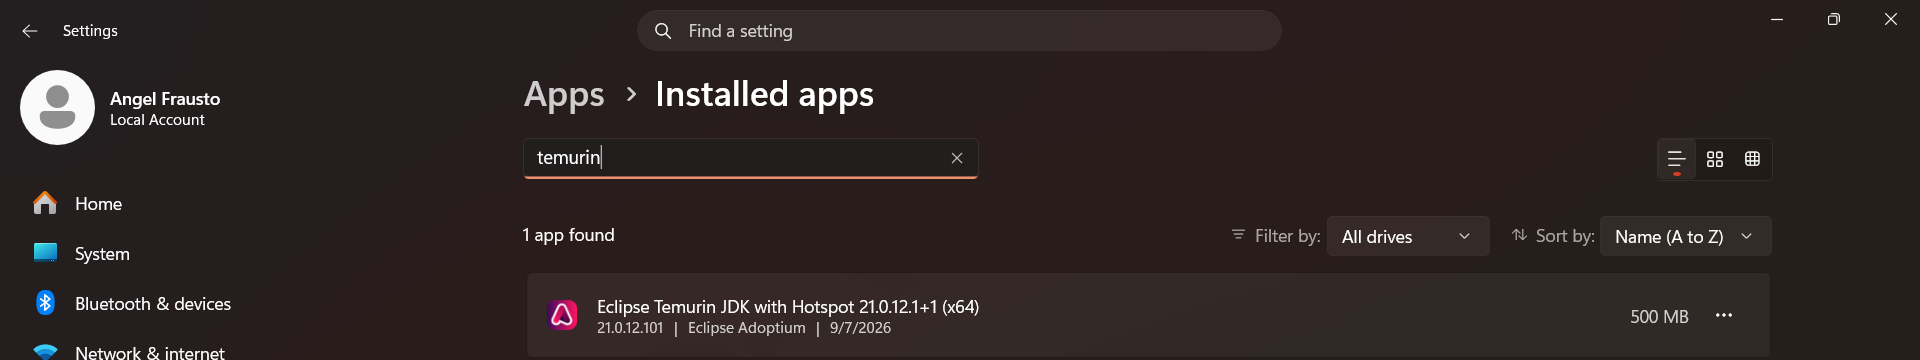
\includegraphics[width=0.85\textwidth]{captura2-instalador.png}
	\caption{JDK registrado en Windows tras la instalación (Configuración $\rightarrow$ Aplicaciones)}
	\label{img:instalador}
\end{figure}

La instalación se realizó con el instalador \texttt{.msi} para Windows, que ejecuta el proceso completo de forma asistida: copia los binarios a \texttt{Program Files}, registra el JDK en el sistema y ofrece la opción de agregarlo automáticamente a la variable \texttt{PATH}. Aun con esa opción activada, es necesario revisar (y, en caso de que falte, declararla a mano) la variable \texttt{JAVA\_HOME}, porque muchas herramientas de compilación (Maven, Gradle) y varios IDEs la consultan directamente en vez de inferirla a partir del \texttt{PATH}. La instalación queda registrada en el sistema y puede confirmarse desde \textit{Configuración $\rightarrow$ Aplicaciones}, donde Windows lista a Eclipse Temurin JDK como programa instalado.

\subsection{ \color{colorESCOM}{Configuración de la variable \texttt{JAVA\_HOME}}}

\begin{figure}[H]
	\centering
	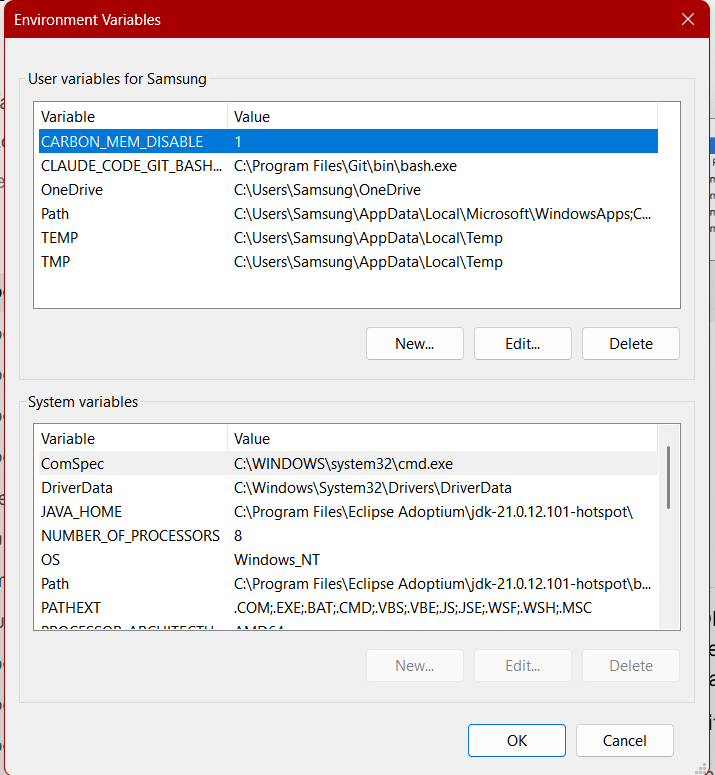
\includegraphics[width=0.85\textwidth]{captura3-variables-entorno.png}
	\caption{Variable de entorno \texttt{JAVA\_HOME} configurada en Windows}
	\label{img:variables}
\end{figure}

En Windows, las variables de entorno se configuran desde \textit{Panel de Control $\rightarrow$ Sistema $\rightarrow$ Configuración avanzada del sistema $\rightarrow$ Variables de entorno} \cite{oracle2024envvar}. Ahí se creó una variable nueva de usuario llamada \texttt{JAVA\_HOME}, cuyo valor apunta a la carpeta raíz de la instalación del JDK (no a la subcarpeta \texttt{bin}, que es el error más común en este paso), y se agregó \texttt{\%JAVA\_HOME\%\textbackslash bin} al final de la variable \texttt{Path}, para que el sistema encuentre los ejecutables \texttt{java} y \texttt{javac} desde cualquier terminal.

\subsection{ \color{colorESCOM}{Verificación}}

Con la variable ya configurada, se abrió una terminal nueva (paso obligatorio: una terminal ya abierta conserva el entorno con el que arrancó y no ve variables agregadas después) y se confirmó la instalación con los comandos \texttt{java -version} y \texttt{javac -version}:

\begin{lstlisting}[caption={Verificación del JDK instalado y de la variable JAVA\_HOME}]
$ java -version
openjdk version "21.0.12.1" 2026-08-18 LTS
OpenJDK Runtime Environment Temurin-21.0.12.1+1 (build 21.0.12.1+1-LTS)
OpenJDK 64-Bit Server VM Temurin-21.0.12.1+1 (build 21.0.12.1+1-LTS, mixed mode, sharing)

$ javac -version
javac 21.0.12.1

$ echo %JAVA_HOME%
C:\Program Files\Eclipse Adoptium\jdk-21.0.12.101-hotspot\
\end{lstlisting}

\begin{figure}[H]
	\centering
	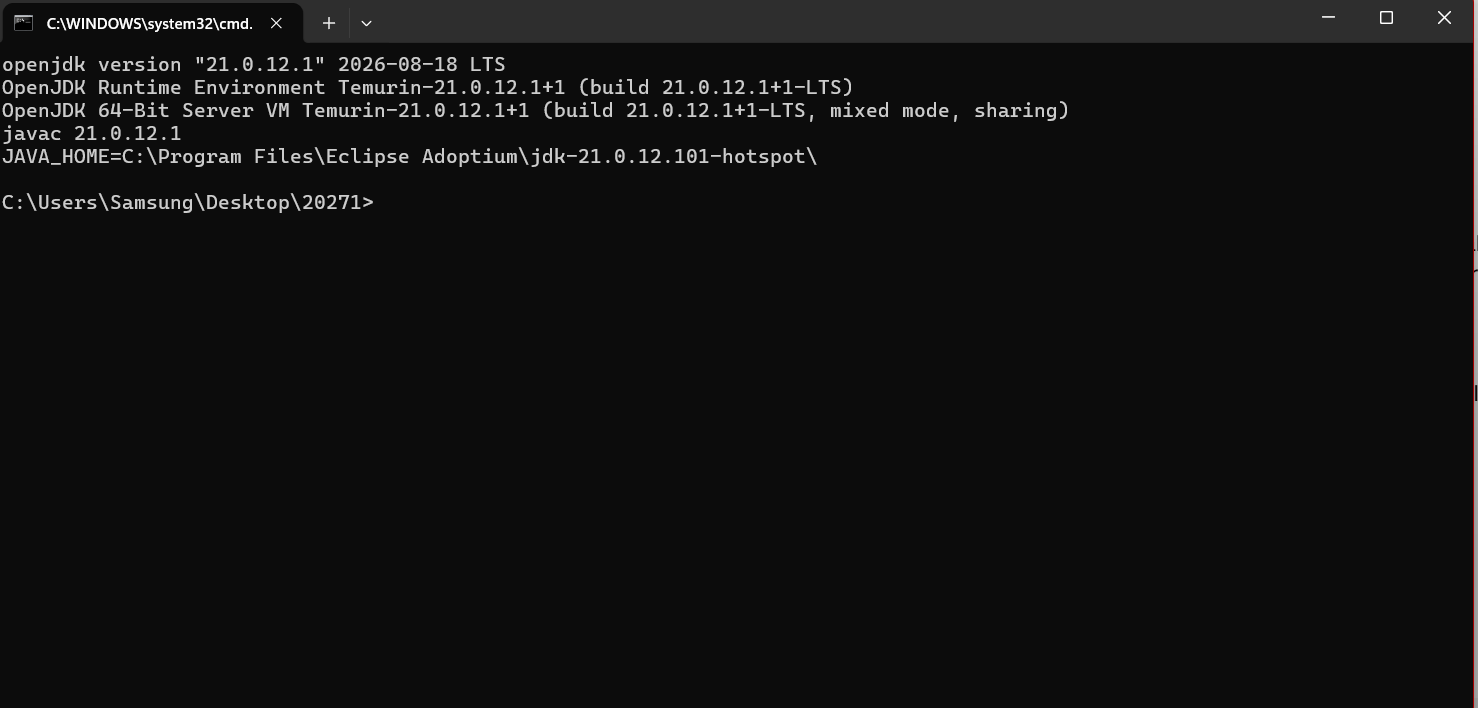
\includegraphics[width=0.85\textwidth]{captura4-verificacion.png}
	\caption{Verificación de \texttt{java -version} y \texttt{JAVA\_HOME} en la terminal}
	\label{img:verificacion}
\end{figure}

Los tres comandos coinciden: la versión que reporta el ejecutable de Java es la misma que la del compilador, y \texttt{JAVA\_HOME} apunta exactamente a la carpeta donde ese ejecutable vive. Esa coincidencia es, en la práctica, la prueba de que la instalación quedó bien encadenada de principio a fin.

%################################################
\section{\color{colorIPN}{Conclusión}}

La instalación del JDK es un proceso corto, pero con varios puntos donde suele fallar, casi siempre por descuido y no por dificultad técnica real. Los más comunes son:

\begin{itemize}
	\item \textbf{Apuntar \texttt{JAVA\_HOME} a la carpeta \texttt{bin} en vez de a la raíz del JDK.} Es el error más frecuente. Herramientas como Maven esperan que \texttt{JAVA\_HOME} sea la carpeta que \textit{contiene} a \texttt{bin}, no \texttt{bin} en sí misma; el síntoma típico es un error de \enquote{no se encuentra el ejecutable} aunque \texttt{java -version} funcione bien desde el \texttt{PATH}.
	\item \textbf{No abrir una terminal nueva después de configurar la variable.} Las variables de entorno se leen una sola vez, al arrancar el proceso. Una terminal o un IDE que ya estaban abiertos antes del cambio van a seguir sin ver \texttt{JAVA\_HOME} hasta que se reinicien.
	\item \textbf{Instalar solo el JRE en vez del JDK.} El JRE (Java Runtime Environment) permite \textit{ejecutar} programas Java pero no trae el compilador \texttt{javac}; para desarrollo hace falta específicamente el JDK.
	\item \textbf{Tener varias versiones del JDK instaladas y que el \texttt{PATH} apunte a una distinta de la que se acaba de configurar en \texttt{JAVA\_HOME}.} Provoca que \texttt{java -version} y \texttt{javac -version} reporten números distintos, lo que suele romper la compilación de forma difícil de diagnosticar si no se revisan ambos comandos por separado.
	\item \textbf{Descargar el instalador de arquitectura equivocada} (32 bits en un sistema de 64 bits, o viceversa), lo que puede impedir la instalación o generar errores de compatibilidad más adelante con otras herramientas de 64 bits del entorno de desarrollo.
\end{itemize}

Verificar con dos comandos distintos (\texttt{java -version} y \texttt{javac -version}) en vez de uno solo, y confirmar el valor de \texttt{JAVA\_HOME} de forma explícita en vez de asumirlo, es la forma más directa de detectar cualquiera de estos problemas antes de que se manifieste como un error confuso en Maven, Gradle o el IDE más adelante en el curso.

%################################################
\pagebreak

\section{\color{colorIPN}{Referencias Bibliográficas}}
\color{colorESCOM}{
	\printbibliography[heading=none]
}

\end{document}
